%  LaTeX support: latex@mdpi.com
%  In case you need support, please attach any log files that you could have,
% and specify the details of your LaTeX setup (which operating system and LaTeX
% version / tools you are using).

%=================================================================

% LaTeX Class File and Rendering Mode (choose one)
% You will need to save the "mdpi.cls" and "mdpi.bst" files into the same folder
% as this template file.

%=================================================================

\documentclass[energies,article,accept,moreauthors,pdftex,12pt,a4paper]{mdpi}

%=================================================================
\setcounter{page}{1}
\lastpage{x}
\doinum{10.3390/------}
\pubvolume{xx}
\pubyear{2015}
\history{Received: xx / Accepted: xx / Published: xx}
%------------------------------------------------------------------
% The following line should be uncommented if the LaTeX file is uploaded to
% arXiv.org
%\pdfoutput=1

%=================================================================

% Add packages and commands to include here
% The amsmath, amsthm, amssymb, hyperref, caption, float and color packages are
% loaded by the MDPI class.
\usepackage{graphicx}
%\usepackage{subfigure,psfig}
\usepackage[draft]{todonotes}

\def \p{\partial}
\def \d{\mathrm{d}}
\def \D{\mathrm{D}}

%=================================================================
%% Please use the following mathematics environments:
%\theoremstyle{mdpi}
%\newcounter{thm}
%\setcounter{thm}{0}
%\newcounter{ex}
%\setcounter{ex}{0}
%\newcounter{re}
%\setcounter{re}{0}
%\newtheorem{Theorem}[thm]{Theorem}
%\newtheorem{Lemma}[thm]{Lemma}
%\newtheorem{Characterization}[thm]{Characterization}
%\newtheorem{Proposition}[thm]{Proposition}
%\newtheorem{Property}[thm]{Property}
%\newtheorem{Problem}[thm]{Problem}
%\newtheorem{Example}[ex]{Example}
%\newtheorem{Remark}[re]{Remark}
%\newtheorem{Corollary}[thm]{Corollary}
%\newtheorem{Definition}[thm]{Definition}
%% For proofs, please use the proof environment (the amsthm package is loaded by
% the MDPI class).

%=================================================================

% Full title of the paper (Capitalized)
\Title{Effects of Reynolds Number on the Performance and Near-Wake Dynamics of a
Vertical-Axis Cross-Flow Turbine}

% Authors (Add full first names)
\Author{Peter Bachant $^{1,}$* and Martin Wosnik $^{1}$}

% Affiliations / Addresses (Add [1] after \address if there is only one
% affiliation.)
\address{%
$^{1}$ Center for Ocean Renewable Energy, University of New Hampshire, 24
Colovos Rd., Durham, NH, USA}

% Contact information of the corresponding author (Add [2] after \corres if
% there are more than one corresponding author.)
\corres{pxL3@unh.edu}

% Abstract (Less than 200 words)
\abstract{The acceptable Reynolds number mismatch for scaled physical model
testing a cross-flow turbine is investigated experimentally, both with respect
to prediction of full-scale performance, and wake characteristics, which will be
drivers of overall performance and interaction between multiple turbines.}

% Keywords: add 3 to 10 keywords
\keyword{keyword; keyword; keyword}

% The fields PACS, MSC, and JEL may be left empty or commented out if not
% applicable
%\PACS{}
%\MSC{}
%\JEL{}

\begin{document}

\listoftodos

\section{Introduction}

Scaled physical models are often used in science and engineering to approximate
real-world systems. However, the principle of dynamic similarity allows for
geometrically scaled systems to be dynamically identical in scale if certain
nondimensional physical parameters are matched. In the case of fluid systems,
the most important parameter is often the Reynolds number, which quantifies the
importance of viscosity on the flow physics. As such, hereafter we will use the
word ``scale'' to refer to this dynamical scale rather than the geometric scale.

With regards to wind and marine hydrokinetic (MHK) turbines, scaled physical
models are used to validate predictive numerical models, predict full-scale
performance of individual turbines, and design or investigate arrays of devices.
Despite being significantly less expensive, there is still some concern at which
scale an experiment must be performed to be relevant to full-scale application.

For numerical models, one might obtain favorable predictions for scaled systems
due to modified physics. If the numerical model is then considered
``validated,'' there is a risk that its application at full-scale may produce
incorrect predictions. For scaled physical prototypes, it is of interest how
small---since size, or scale generally correlates inversely with cost---the
prototype can be while remaining a reliable predictor of full-scale behavior. At
the very least, it is necessary to test at a scale where results can be
extrapolated, i.e. changes are occurring quasi-linearly without dramatic changes
in the underlying physical principles governing the behavior of interest, e.g.
power production in the case of a wind or MHK turbine.

Blackwell et al. investigated the effects of Reynolds number on the performance
of a 2 m diameter Darrieus vertical-axis cross-flow wind turbine with NACA 0012
blades \cite{Blackwell1976}. By varying wind tunnel speed, the turbine was made
to operate at approximately constant blade chord Reynolds number $Re_c$ ranging
from $1 \times 10^5$ to $3 \times 10^5$. In this regime the turbine power
coefficient $C_P$ was shown to be sensitive to $Re_c$, with sensitivity
diminishing at the higher Reynolds numbers, especially for turbines of lower
solidity ($Nc/R$, where $N$ is the number of blades and $R$ is the turbine's
maximum radius). More recently, Polagye and Cavagnaro observed high Reynolds
number sensitivity for a high solidity helical cross-flow turbine
\cite{Polagye2013b}, and Bravo et al. observed power coefficient of a
straight-bladed VAWT to become Reynolds number independent at $Re_c \approx 4
\times 10^5$.

When designing or studying arrays, it is common to use very small
(geometrically) scaled devices \cite{Chamorro2011, Chamorro2011b}. It is
therefore important to realize the limitations of evaluating both the power
output of turbines and the wake recovery when Reynolds number is very far from
full scale. Sometimes models used are not turbines, but wake generating objects,
e.g., porous disks, that are meant to replicate the wakes of real turbines
\cite{Goldenberg1983}. In this case, it is of interest to determine at what
scale one might be able to realistically study wake flows in an array, and also
to evaluate the effectiveness of a wake generator. In other words, a wake
generator may do a fine job simulating a scaled turbine, but how well can it
simulate a full-scale device?

Previously, is has been observed experimentally that a cross-flow turbine wake's
unique vortical mean flow field is responsible for accelerated wake recovery
when compared with conventional axial-flow propeller-type turbines
\cite{Bachant2015-JoT}. In this study we seek to replicate the same energy
balance considerations at multiple Reynolds numbers, to examine the implications
on how small scale, i.e. low Reynolds number experiments may be used to study
flows in turbine arrays.

The Reynolds number effects on the maximum performance and 2-D near-wake
profiles of the University of New Hampshire's Reference Vertical Axis Turbine
(UNH-RVAT) were presented \cite{Bachant2014}. In this study we set out to
analyze in greater depth the effects of scale, i.e. Reynolds number, on the
performance of the turbine, and its more detailed near-wake characteristics. We
were looking to find a threshold scale beyond which a physical model study could
reliably predict full-scale performance. We were also looking to investigate the
sensitivity as small scales, and what the implications might be for validating
the prediction capabilities of numerical models.

\todo[inline]{Talk about interdependence of Froude number.}

\subsection{Reynolds Number Effects}

In this study we are focused on a turbine constructed from foils---a lift-driven
device in contrast to drag-driven. A logical starting point for understanding
the effects of $Re$ on overall turbine loading is to look at simplified cases
of individual foils, with respect to their static and dynamic loading. 

\subsubsection{On Static Foil Behavior}

Blade performance is generally characterized by the lift-to-drag ratio $l/d$,
which is a function of the foil's angle of attack $\alpha$. The angles of attack
for cross-flow turbine blades are a function of turbine tip speed ratio,
induction (slowing/turning of the free stream flow prior to reaching the
turbine), and turbine rotation or azimuthal angle $\theta$. Looking at static
airfoil data, we see that the static stall angle---the angle just beyond that at
which $l/d$ is maximum---increases with blade chord Reynolds number $Re_c$. This
in general is caused by the blade boundary becoming more turbulent as a fraction
of the chord length, diminishes the negative effects of a laminar separation
bubble occurring near the leading edge. For smooth airfoils, this transition can
cause a dramatic increase in foil performance, a shown in
Figure~\ref{fig:McMasters} at a blade chord Reynolds number on the order of
$10^5$ \cite{McMasters1980}. A review of low Reynolds number airfoil behavior is
presented in \cite{Lissaman1983}. Note that there is a distinct lack of highly
reliable data for airfoils in this transitional regime and below. An evaluation
of the various databases relevant to cross-flow turbines is presented in
\cite{Bedon2014}.

\begin{figure}[ht]
\centering
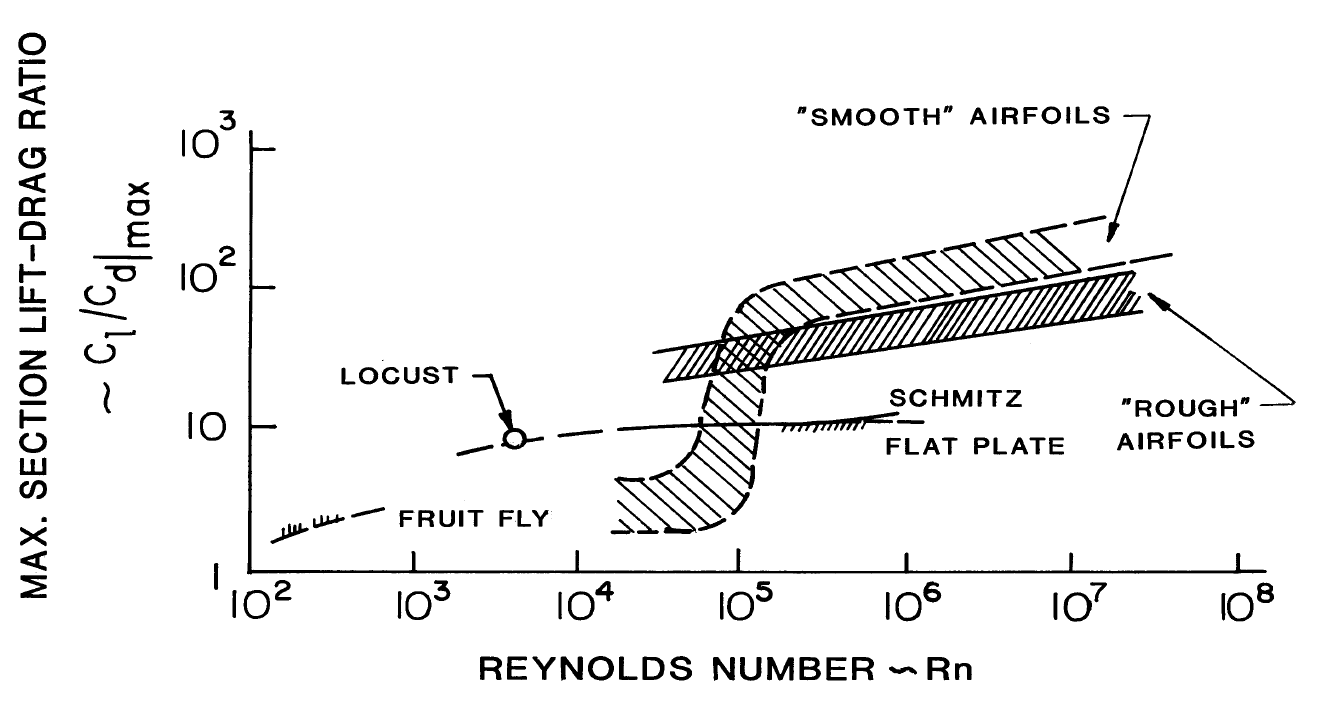
\includegraphics[width=0.7\textwidth]{figures/McMasters-Henderson-1980}
\caption{Airfoil lift to drag ratio as a function of Reynolds number, from 
\cite{McMasters1980}.}
\label{fig:McMasters}
\end{figure}

\subsubsection{On Dynamic Foil Behavior}

Static foil performance does not tell the whole story for a cross-flow turbine.
The azimuthal, and therefore temporal variation of $\alpha$ in a cross-flow
turbine implies dynamic loading. Furthermore, the blades commonly undergo
dynamic stall for tip speed ratios at and below those of maximum rotor
torque\cite{Para2002}. We then must understand the effects of Reynolds number on
the dynamic stall process.

Dynamic effects on blade loading can be distinguished between attached and
separated conditions. 

\todo[inline]{Find reference to describe $Re$ effects on dynamic foil behavior.}

Bousman showed that dynamic stall was insensitive to Reynolds number for $Re=1.0
\times 10^5$--$2.5 \times 10^5$ \cite{Bousman2000-evaluation}.

\subsubsection{On Wake Flows}

We expect that lower lift on the blades at lower $Re$ will weaken tip vortex
shedding, and decrease the levels of turbulence shed from the blade boundary
layers. As mentioned previously, the dynamic stall vortex shedding is not
expected to have a large Reynolds number sensitivity, though a larger separation
bubble at lower $Re$ may induce higher levels of turbulence as shed vortices
become unstable and break down.

\todo[inline]{What do studies in the literature tell us about $Re$ effects
on shear flows, wakes, and vortex flows?}

Chamorro et al. showed that turbulence statistics in an AFT wake became
$Re$-independent at $Re_D \approx 1 \times 10^5$, with mean velocity slightly
earlier at $Re_D \approx 5 \times 10^4$ \cite{Chamorro2012}.

\section{Experimental Setup}

Experiments were performed in the University of New Hampshire's tow/wave tank
turbine test bed. The turbine model is dubbed the UNH-RVAT, for Reference
Vertical Axis Turbine, which is designed to be a generic case for numerical
model testing, similar to the Sandia National Labs/US Department of Energy RM2
River Turbine, but with higher solidity, or blade chord to radius ratio. A CAD
model of the turbine, depicted in \ref{fig:turbine}, is available from
\cite{Bachant2014-RVAT-CAD}.

\begin{figure}[ht!]
\centering
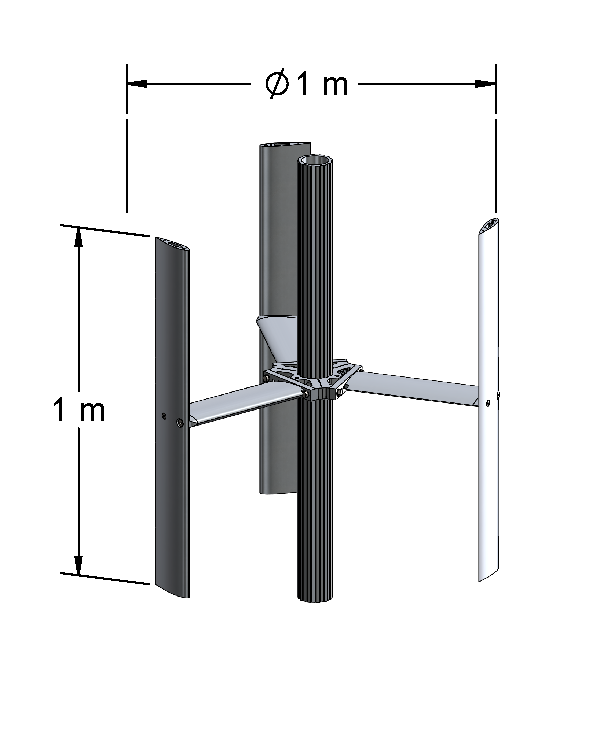
\includegraphics[width=0.4\textwidth]{figures/turbine}
\caption{Turbine model drawing. Note that the upper and lower mounting
flanges have been excluded as these were included in the tare drag
measurements.} 
\label{fig:turbine}
\end{figure}


The turbine was mounted in a frame constructed from NACA 0020 sections. The
turbine shaft ran up through the water surface, coupled to a permanent magnet
servo motor with a 20:1 gearbox. This servo was controlled by the tow tank's
main motion controller for high synchronization with the carriage motion. A
rotary torque transducer was installed inline between the servo and the turbine,
and the servo was also mounted on a slewing ring bearing, which allowed a
redundant measurement of torque via an arm and load cell used to counteract the
turbine moment. The frame was mounted to the carriage via linear guides, such
that the total streamwise drag force was transferred to a pair of S-beam load
cells, providing the rotor drag measurements, after a measured tare drag was
subtracted in post processing. Similarly, a tare torque was measured by rotating
the turbine shaft in air. Turbine angular and tow carriage linear position were
measured using quadrature encoder signals, with $10^5$ counts-per-rev for the
turbine and 10 $\mathrm{\mu m}$ resolution for the carriage position. These
signals, along with the torque and drag signals, were sampled at 2 kHz.

\begin{figure}[ht!]
\centering
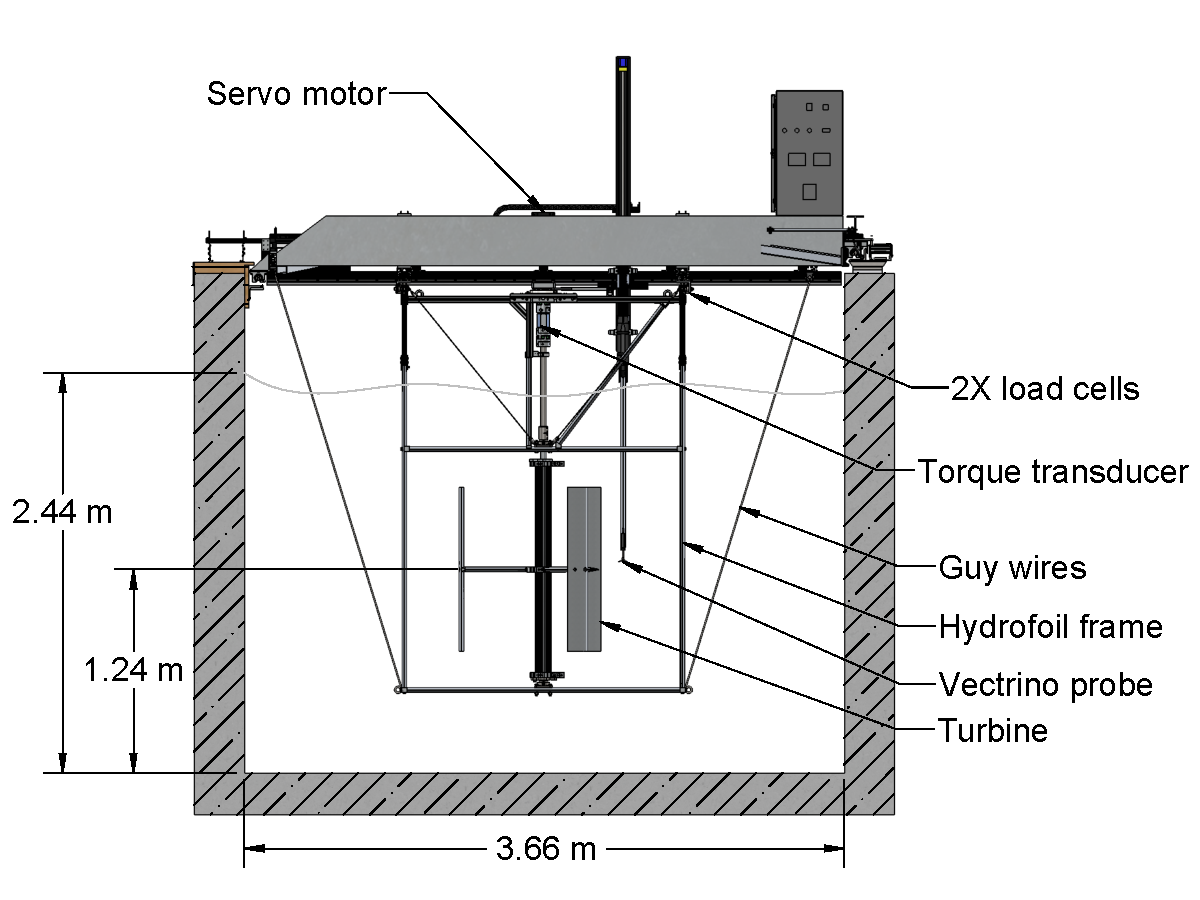
\includegraphics[width=0.75\textwidth]{figures/exp_setup_drawing}
\caption{Drawing of the experimental setup.}
\label{fig:exp-setup}
\end{figure}

Wake velocity was measured using a Nortek Vectrino+ acoustic Doppler velocimeter
(ADV), sampling at 200 Hz. The probe was mounted on an automated positioning
system, also controlled by the tow tank's main motion controller. The ADV and
DAQ systems' sampling times were synchronized by triggering the start of data
acquisition via a pulse sent from the motion controller.

\subsection{Test Plan} 

Approximately 1500 tows were performed, each one used for a single data point on
either a performance curve or wake map. A performance curve consisted of 31
tows, where during each tow the mean turbine tip speed ratio was held constant,
ranging from 0.1--3.1 in 0.1 increments. Full performance curve data were
acquired for tow speeds from 0.4 to 1.2 m/s in 0.2 m/s increments, for which
turbine diameter and approximate blade chord Reynolds number are presented in
Table~\ref{tab:Re}. Performance was also measured for $\lambda=1.9$ at tow
speeds $[0.3, 0.5, 0.7, 0.9, 1.1, 1.3]$ m/s for two tows each.

\begin{table}
\centering
\begin{tabular}{ccc}
Tow speed (m/s) & $Re_D$ & $Re_{c,\mathrm{ave}}$ ($\lambda = 1.9$) \\ 
\hline
0.3 & $3.0 \times 10^5$ & $8.0 \times 10^4$ \\ 
0.4 & $4.0 \times 10^5$ & $1.1 \times 10^5$ \\ 
0.5 & $5.0 \times 10^5$ & $1.3 \times 10^5$ \\ 
0.6 & $6.0 \times 10^5$ & $1.6 \times 10^5$ \\ 
0.7 & $7.0 \times 10^5$ & $1.9 \times 10^5$ \\ 
0.8 & $0.8 \times 10^5$ & $2.1 \times 10^5$ \\ 
0.9 & $0.9 \times 10^5$ & $2.4 \times 10^5$ \\ 
1.0 & $1.0 \times 10^6$ & $2.7 \times 10^5$ \\ 
1.1 & $1.1 \times 10^6$ & $2.9 \times 10^5$ \\ 
1.2 & $1.2 \times 10^6$ & $3.2 \times 10^5$ \\ 
1.3 & $1.3 \times 10^6$ & $3.4 \times 10^5$ \\ 
\end{tabular} 
\caption{Turbine diameter and approximate blade chord Reynolds numbers for the
tow speeds used in the experiment.}
\label{tab:Re}
\end{table}

A wake map was generated by positioning the Vectrino probe at 270 different
locations, varied in the cross-stream and vertical directions at one turbine
diameter downstream ($x/D=1$). These locations have vertical coordinates from
the turbine centerline up to $z/H=0.625$, ranging in the cross-stream direction
$y/R = \pm 3$. These locations are shown in Figure~\ref{fig:wake-locations}.

\begin{figure}
\centering
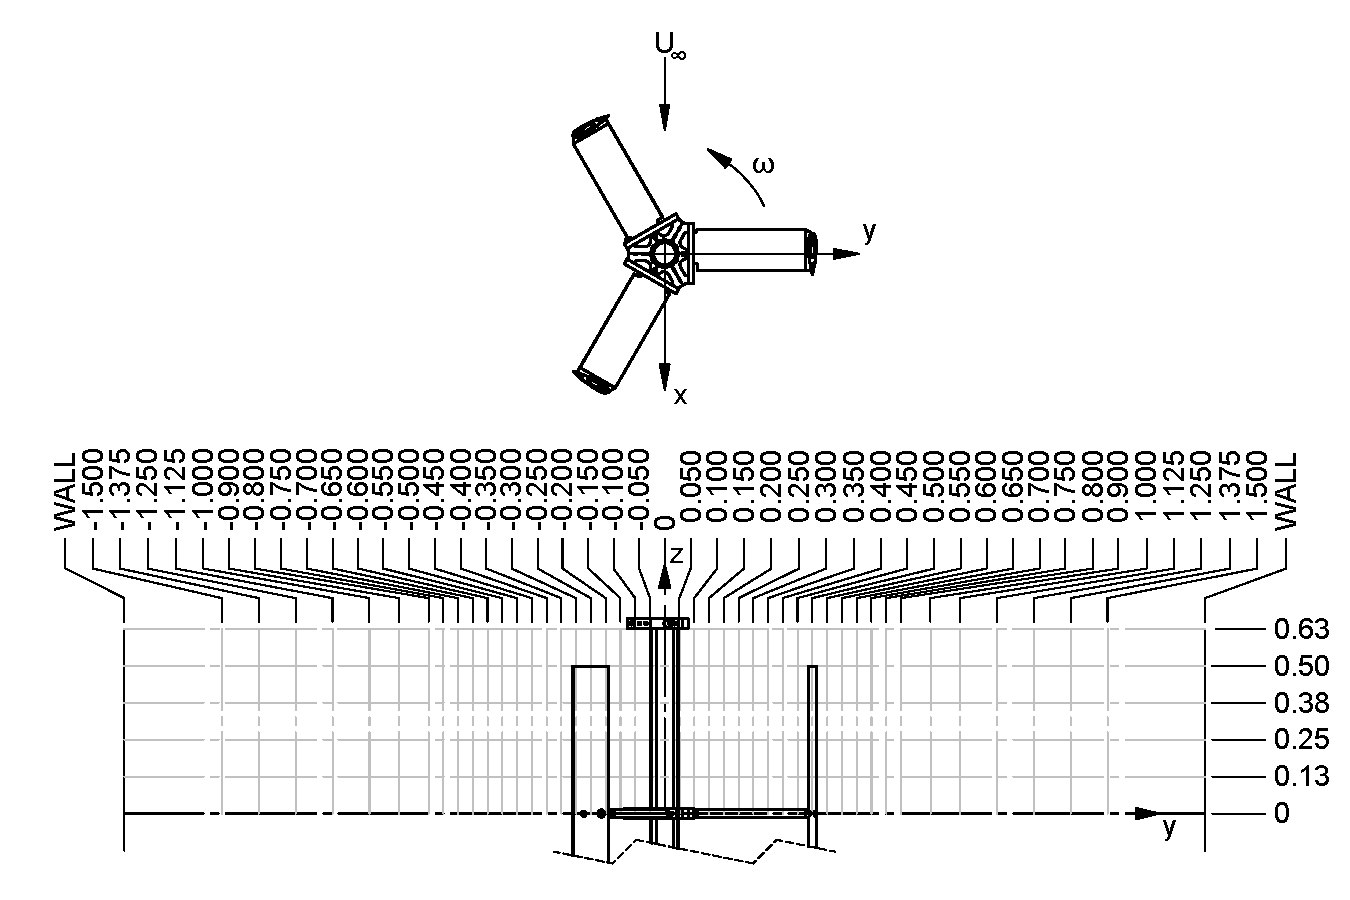
\includegraphics[width=0.9\textwidth]{figures/turbine_coordinate_system}
\caption{Wake measurement coordinate system and locations. Dimensions are in
meters.} 
\label{fig:wake-locations}
\end{figure}

\subsection{Data Processing}

From each set of tows, a standard time interval was set, which allowed the
turbine performance and wake to reach a quasi-periodic state. Each run was
analyzed to compute statistics over this interval, truncating the end slightly
to achieve and integer number of blade passages. Turbine shaft angular velocity
and tow carriage speed were calculated using a second order central differencing
scheme on the respective position measurements. Power and drag coefficients are
calculated as instantaneous quantities using the carriage speed as the free
stream velocity. 

Wake velocity data were filtered for spurious ``spikes'' by removing datapoints
8 standard deviations or 0.9 m/s from the mean. The experimental data and code
for processing and visualization are available from
\cite{Bachant2015-RVAT-Re-dep-data}.


\section{Results and Discussion}


\subsection{Performance}

Full performance curves for various Reynolds numbers are plotted in
Figure~\ref{fig:perf-curves}. There is essentially no change in the shape of the
drag coefficient curves---merely an upward shift in $C_D$ with increasing $Re$.

In general, maximum $C_P$ increases with Reynolds number, which is due to an
increase in the foil lift-to-drag ratio. The power coefficient curves also show
a downward shift in the optimal tip speed ratio with increasing Reynolds number.
This is caused by the stall delay from a more turbulent boundary later on the
blade suction side.

\begin{figure}[ht]
\centering
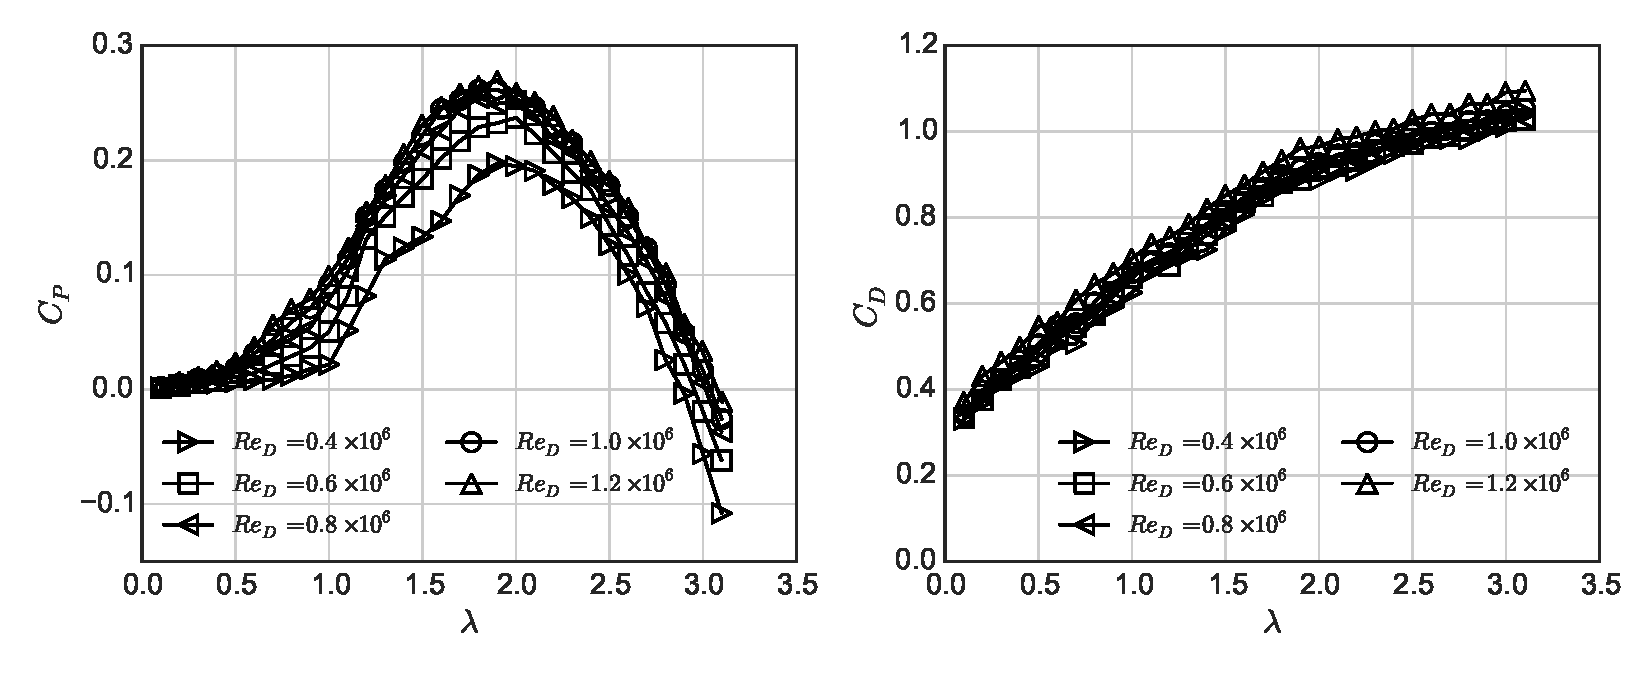
\includegraphics[width=0.95\textwidth]{figures/perf_curves}
\caption{Mean power (left) and drag (right) coefficient curves plotted for
multiple Reynolds numbers.}
\label{fig:perf-curves}
\end{figure}

Mean power and drag coefficients at $\lambda=1.9$ are plotted for all Reynolds
numbers in Figure~\ref{fig:perf-Re-dep}. There is a drastic improvement in $C_P$
with increasing Reynolds number for the lower values. Power coefficient then
becomes  essentially $Re$-independent at $Re_D = 0.8 \times 10^6$, which
corresponds to an approximate average blade chord Reynolds number $Re_{c,
\mathrm{ave}} = 2.1 \times 10^5$. This threshold is consistent with the behavior
of the blade boundary layer transitioning from laminar to turbulent, thereby
promoting reattachment of the laminar separation bubble.

The behavior of the mean rotor drag coefficient is similar, though the changes
are less dramatic. This is likely due to cross-flow turbine geometry, where
increases in blade drag at lower $Re$ somewhat offset the reduction in lift, to
keep total streamwise force from changing as much as the rotor torque. The
tendency for $C_D$ to continue increasing with $Re$ may also be a consequence of
increasing Froude number, which therefore increases free surface deformation and
wave drag during towing without increasing flow through the turbine.

\begin{figure}[ht]
\centering
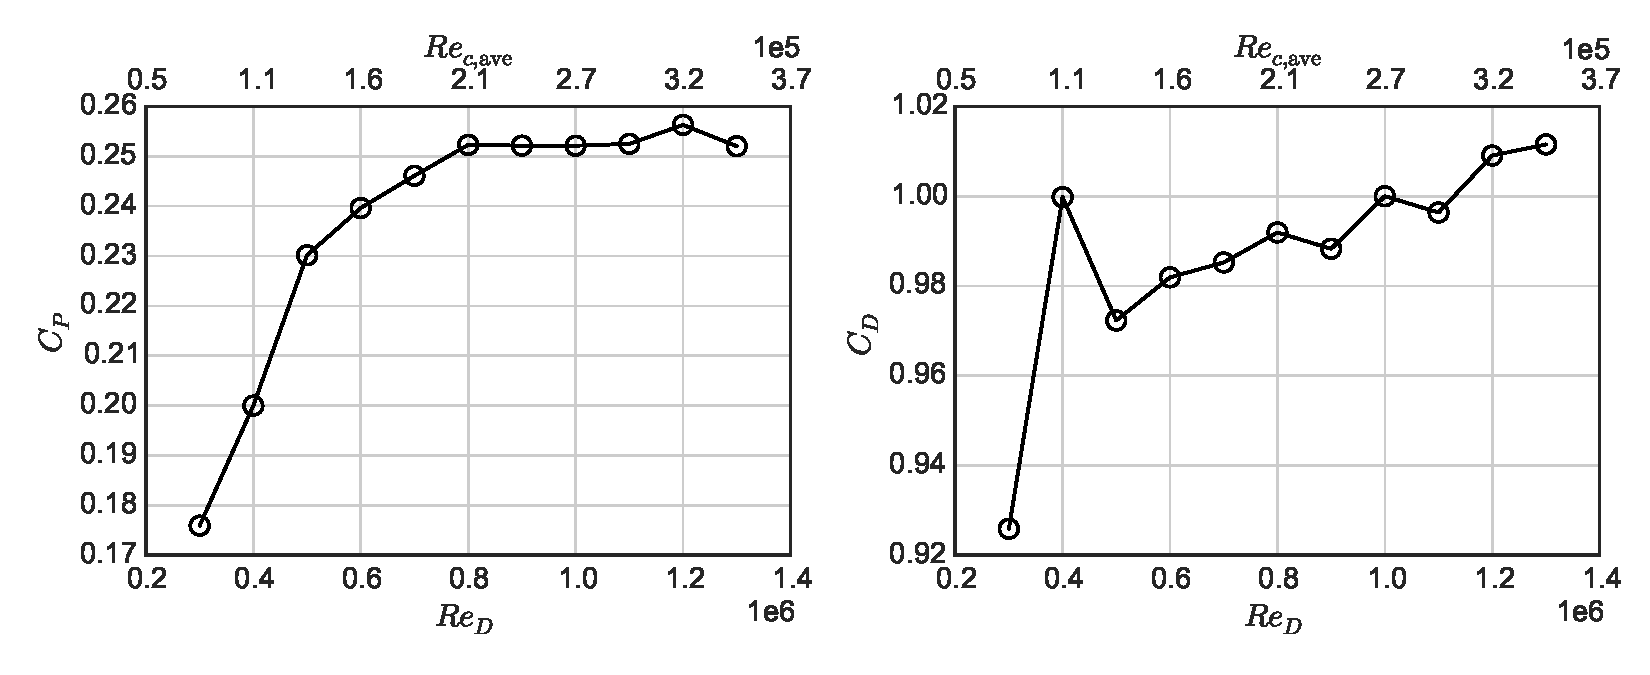
\includegraphics[width=0.95\textwidth]{figures/perf_re_dep}
\caption{Mean power (left) and drag (right) coefficients at $\lambda=1.9$
plotted versus Reynolds number.} 
\label{fig:perf-Re-dep}
\end{figure}

\subsubsection{Relation to Static Foil Characteristics}

To help understand---and possibly predict---the $Re$-sensitivity on turbine
performance, a series of static foil coefficient datasets were computed with the
XFOIL viscous panel method code \cite{Drela1989}, implemented as part of the
open source turbine design software QBlade. Simulations were run with the
default settings and zero Mach number, for the approximate average blade chord
Reynolds numbers encountered in the experiments.

To investigate the effects of the blades' ``virtual camber'' due to their
circular path \cite{Migliore1980}, the XFOIL calculations were performed for
20\% thick foils with 0\% (NACA 0020), 2\% (NACA 2520), and 4\% (NACA 4520)
camber about their half-chord location. A 4\% camber approximates the maximum
distance between the blade chord line and path for the UNH-RVAT and the 2\%
camber takes into account the reduction in virtual flow curvature from the
non-curved inflow velocity by dividing by the tip speed ratio $\lambda=1.9$.

Results from the XFOIL calculations are shown in Figure~\ref{fig:foil-Re-dep},
where values of maximum lift coefficient, minimum drag coefficient, and maximum
lift-to-drag ratio are normalized (for comparison between foils) and plotted
versus $Re_c$. In general, larger camber is associated with decreased foil
performance at lower Reynolds number.

\begin{figure}[ht!]
\centering
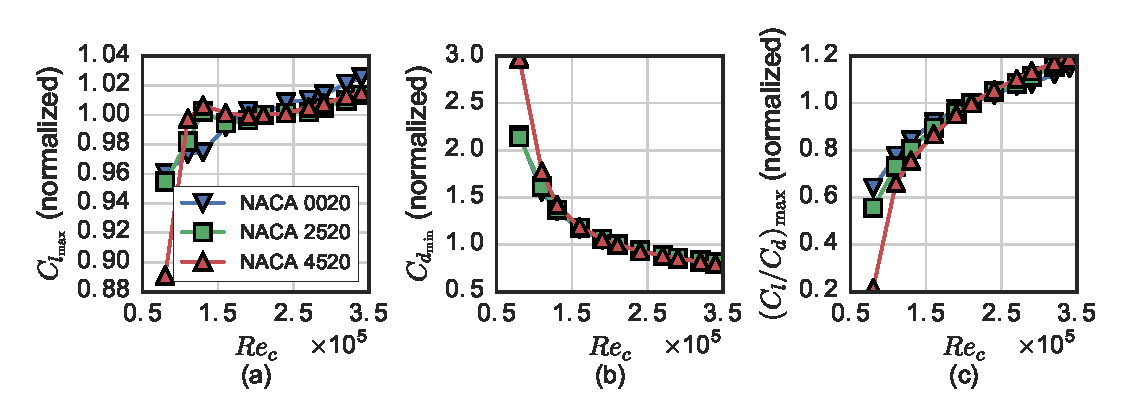
\includegraphics[width=0.95\textwidth]{figures/all_foils_re_dep}
\caption{Foil section characteristics computed by XFOIL for various $Re_c$.}
\label{fig:foil-Re-dep}
\end{figure}

In conjunction with the cross-flow turbine blade kinematics, the foil
coefficients were used to approximate turbine performance by calculating the
peak torque coefficient on the upstream half of the blade path. The turbine
torque coefficient $C_T$ can be related to the blade section chordwise force
coefficient $C_c$ by
\begin{equation}
C_T = \frac{C_c c}{2R} \frac{|U_\mathrm{rel}|^2}{U_\infty^2},
\end{equation}
where the blade section chordwise force (for zero preset pitch)
\begin{equation}
C_c = C_l \sin \alpha - C_d \cos \alpha.
\end{equation}

The relative blade velocity was calculated by adding the free stream to the
opposite of the blade tangential velocity. Note that this neglects any
induction, or slowing of the free stream by the turbine forces, which would be
present in a momentum/streamtube model. Since we were not looking to predict
absolute performance but rather relative changes with $Re$, this method was
deemed acceptable as it is extremely simple and fast to compute. 

Values for the blade angle of attack, relative velocity, and torque coefficient
are plotted in Figure~\ref{fig:blade-kinematics}. The effects of static stall
are clearly present in the torque coefficient plot, and by the time the angle of
attack has decreased below that of stall, the relative velocity is so low that
there is not much contribution to the torque coefficient.

\begin{figure}[ht!]
\centering
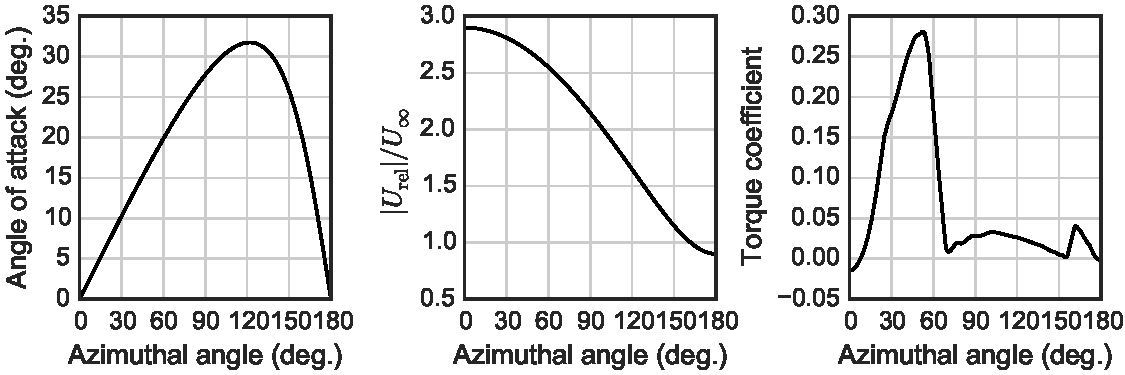
\includegraphics[width=0.95\textwidth]{figures/foil_kinematics_ct}
\caption{Geometric angle of attack (a), relative velocity (b) and torque coefficient
(c) calculated with a NACA 0020 foil.}
\label{fig:blade-kinematics}
\end{figure}

Results for the peak torque coefficient for each foil are plotted versus $Re_c$
in Figure~\ref{fig:foils-C_T-Re-dep}. It is interesting that the convergence of
$C_{T_\mathrm{max}}$ with increasing Reynolds number is more dramatic than any of the
common foil characteristics plotted in Figure~\ref{fig:foil-Re-dep}, meaning
that the cross-flow turbine's unique kinematics must be taken into account when
attempting to predict the effect of transitional Reynolds numbers on turbine
performance. 

From the peak torque coefficient metric, the Reynolds number independence is
achieved at lower values, and more dramatically. We see that the trend of the
NACA 0020 curve matches almost perfectly at low $Re$, but the trend to continue
increasing linearly is not matched by the experimental data, which looks to
behave more like the cambered foil results. Though this method is very
approximate, it nevertheless appears to be a reasonable way to predict the
transitional Reynolds number regime for cross-flow turbine performance using
only 2-D static airfoil characteristics

\begin{figure}[ht!]
\centering
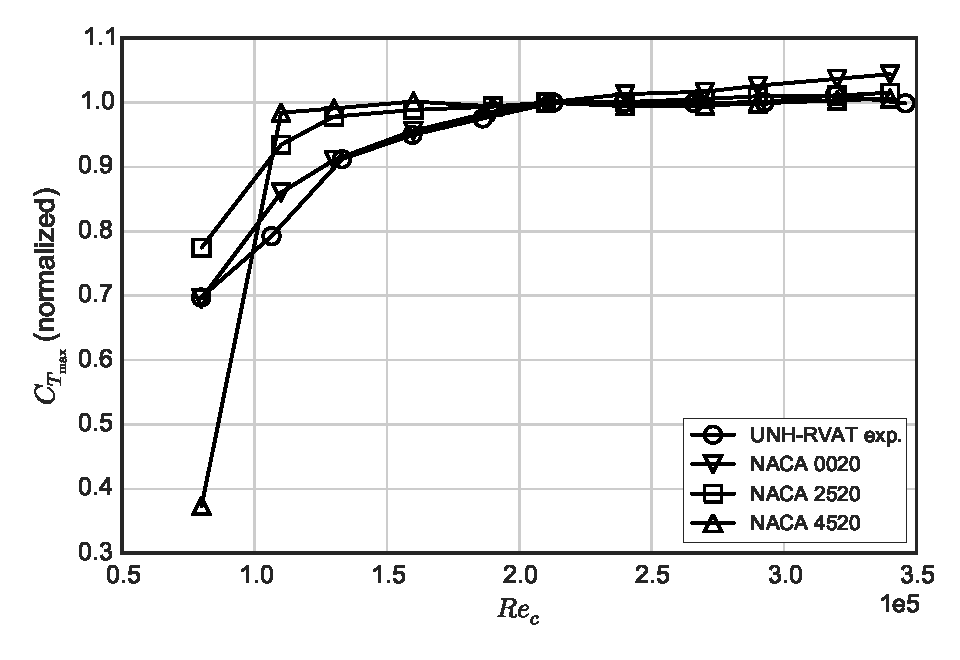
\includegraphics[width=0.65\textwidth]{figures/cft_re_dep_foils}
\caption{Reynolds number dependence of the peak torque coefficient calculated using 
only static foil coefficients and blade kinematics.}
\label{fig:foils-C_T-Re-dep}
\end{figure}


\subsection{Wake Characteristics}

The wake of this turbine at $x/D=1$, $\lambda=1.9$, $Re_D = 1.0 \times 10^6$ was
described thoroughly in \cite{Bachant2015-JoT}. Similar data were taken for the
experiment here, the results for the mean velocity field and turbulence kinetic
energy are shown in Figure~\ref{fig:meancontquiv} and Figure~\ref{fig:kcont},
respectively. With respect to the mean velocity field, we see asymmetry and a
mean vortex structure created by the blade tip vortex shedding. The effects of
the tip vortices are also seen in the turbulence kinetic energy measurements,
along with turbulence generated by the blades undergoing dynamic stall on the
$-y$ side of the turbine.

These same wake maps were taken for $Re_D = 0.4 \time 10^6$, $0.6 \times 10^6$,
$0.8 \times 10^6$, and $1.2 \times 10^6$. Qualitatively, these look strikingly
similar, so they have not been plotted here. We will instead compare and
contrast the wake behavior by examining spectra and wake transport terms in the
equations that govern the downstream evolution.

\begin{figure}[ht!]
\centering
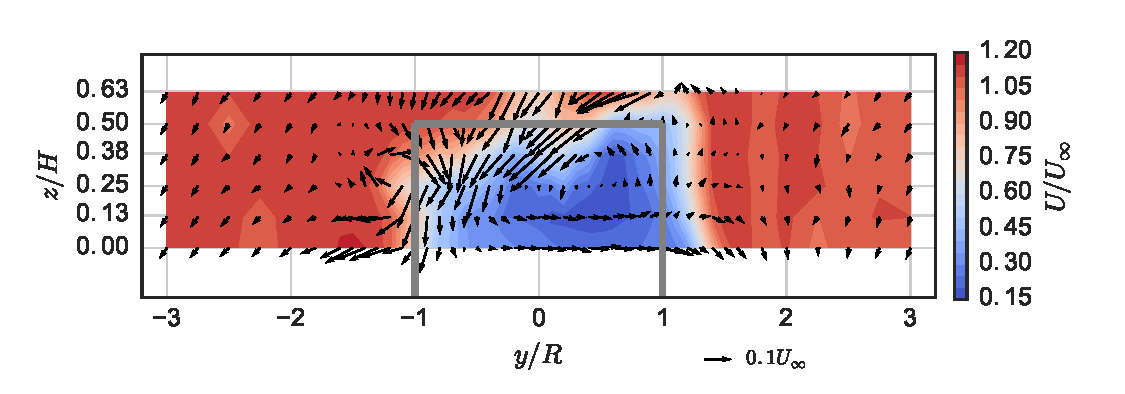
\includegraphics[width=0.8\textwidth]{figures/meancontquiv_10}
\caption{Mean velocity field at $x/D=1$, $\lambda=1.9$, and $Re_D=1.0 \times 10^6$.}
\label{fig:meancontquiv}
\end{figure}

\begin{figure}[ht!]
\centering
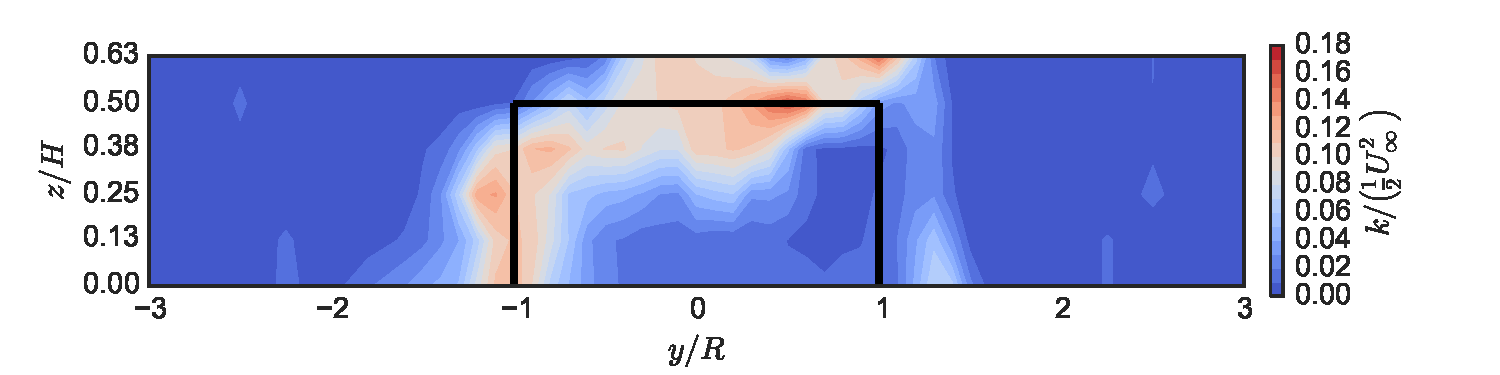
\includegraphics[width=0.8\textwidth]{figures/k_contours_10}
\caption{Turbulence kinetic energy at $x/D=1$, $\lambda=1.9$, and 
$Re_D=1.0 \times 10^6$.}
\label{fig:kcont}
\end{figure}


\subsubsection{Dominant Timescales and Turbulence Spectra}

Spectra of the cross-stream velocity normalized by the free stream are plotted
in Figure~\ref{fig:wake-spectra} for regions on either side of the turbine. On
the $-y$ side of the turbine there is broadband turbulence produced by blade
stall, and on the $+y$ side there is a clear peak in the spectra caused by the
blade passage. We see that on both sides there is higher spectral energy at
lower Reynolds numbers. On the $+y$ side of the turbine we notice higher
spectral energy at the blade passage frequency's first harmonic, or $6
f_\mathrm{turbine}$.

\todo[inline]{Look at how spectra change when turbine rotational frequency
changes relative to inertial subrange.}

\todo[inline]{Make sure the spectra are not just shifting due to normalizing the
noise.}

\begin{figure}[ht!]
\centering
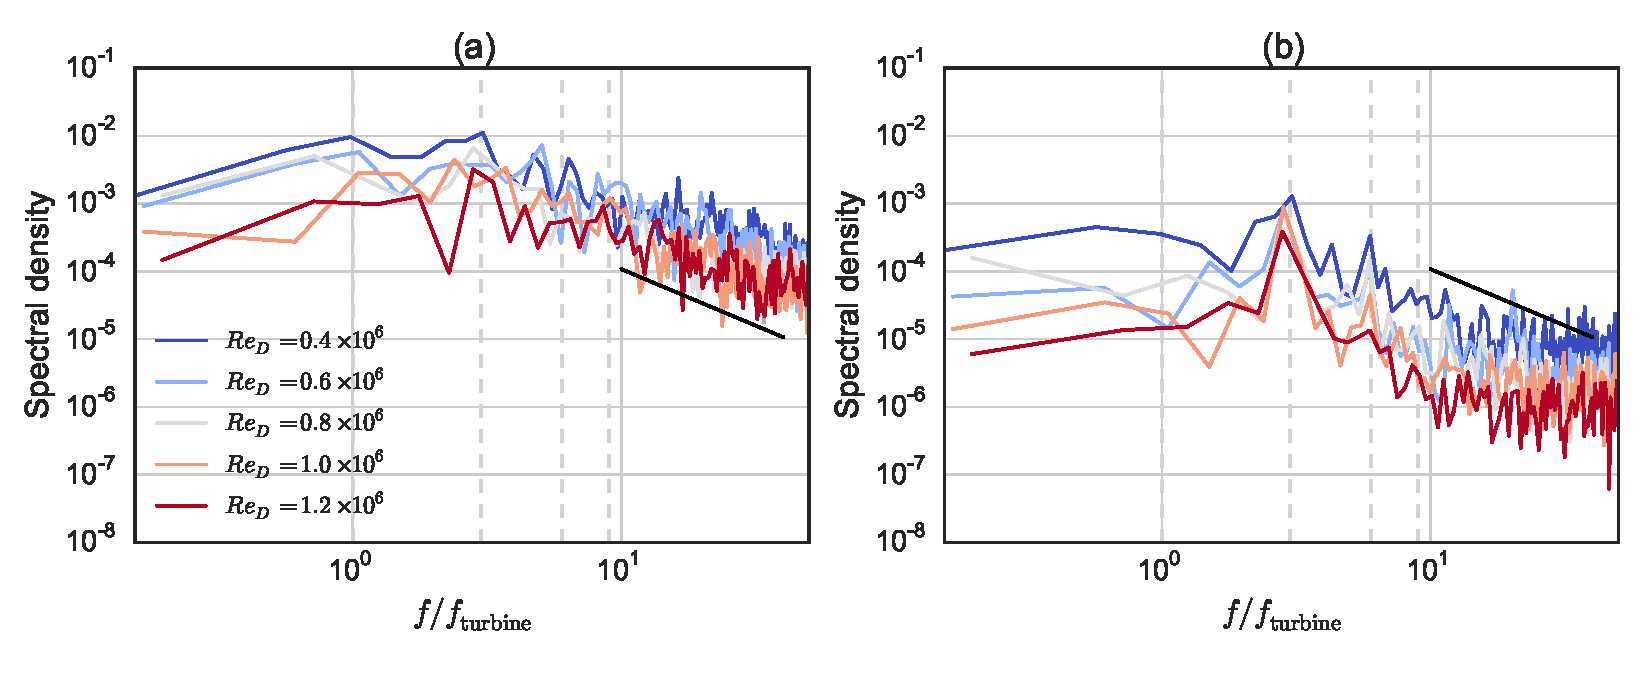
\includegraphics[width=0.95\textwidth]{figures/wake_spectra}
\caption{Cross-stream velocity (normalized by $U_\infty$) spectra at $z/H=0.25$, 
$y/R=-1.0$ (a) and $y/R=1.5$ (b). Dashed vertical
lines indicate $[1, 3, 6, 9]$ times the turbine rotational frequency.}
\label{fig:wake-spectra}
\end{figure}



\subsubsection{Transport of Mean Momentum and Kinetic Energy}

The relative importance of various physical processes on mean streamwise
momentum and kinetic energy transport/recovery in the streamwise direction are
plotted in Figures~\ref{fig:mom-bar-graph} and \ref{fig:K-bar-graph},
respectively. We note that similar to \cite{Bachant2015-JoT}, the vertical
advection at this point in the wake is the dominant contributor to positive wake
recovery, caused by the unique vortex pattern created by the blade tips and
wakes.

We see that in general, levels of turbulent transport are slightly lower at
lower Reynolds numbers. The viscous diffusion and dissipation, though still
three orders of magnitude smaller than the other terms, do increase at low
Reynolds numbers, which is consistent with the definition of the Reynolds number
in general.

\todo[inline]{At what $Re$ will the viscous terms get large enough to start
messing with the balance of the equation?}

\begin{figure}[ht!]
\centering
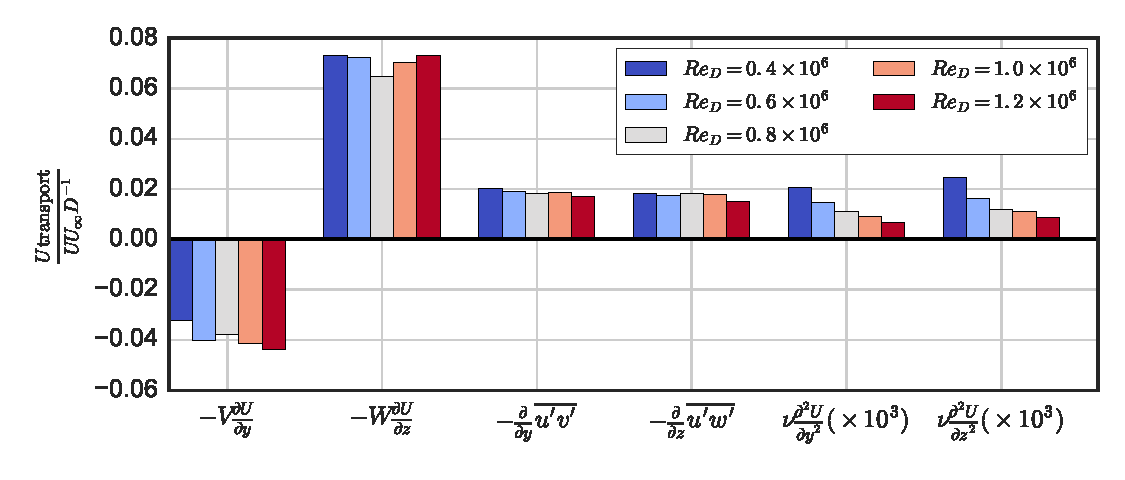
\includegraphics[width=0.9\textwidth]{figures/mom_bar_graph}
\caption{Momentum transport quantities.}
\label{fig:mom-bar-graph}
\end{figure}

\begin{figure}[ht!]
\centering
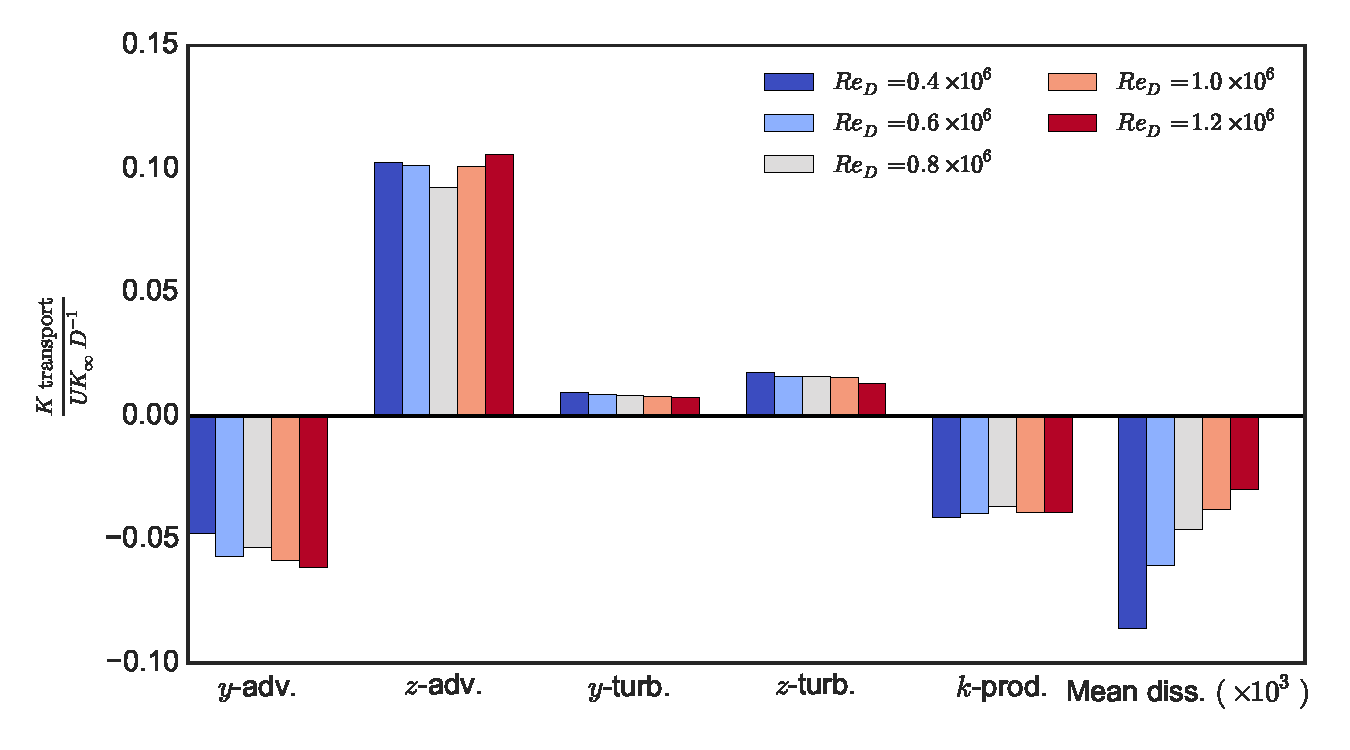
\includegraphics[width=0.9\textwidth]{figures/K_trans_bar_graph}
\caption{Mean kinetic energy transport quantities.}
\label{fig:K-bar-graph}
\end{figure}


Totals for all the wake transport terms calculated are plotted in
Figure~\ref{fig:wake-trans-totals}. We see that in general wake transport is
enhanced at lower Reynolds numbers and levels off consistent with the behavior
of the  turbine power coefficient. This is an important consideration if
studying sub-scale models of turbine arrays, where increased levels of wake
recovery will motivate different ideal array configurations when compared with
full-scale turbines.


\begin{figure}[ht!]
\centering
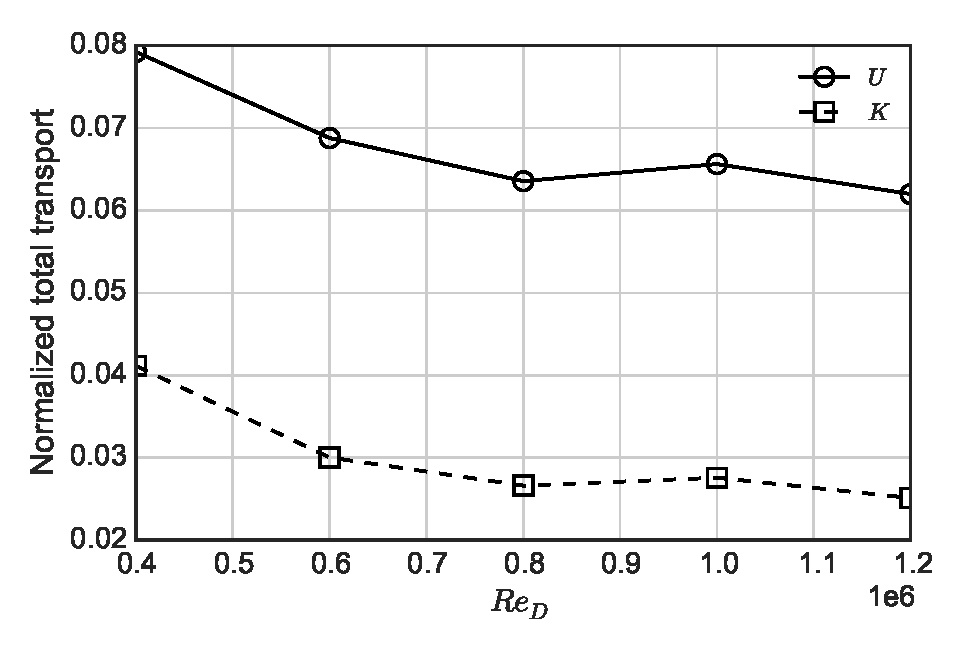
\includegraphics[width=0.65\textwidth]{figures/wake_trans_totals}
\caption{Normalized transport totals from Figures~\ref{fig:mom-bar-graph} and 
\ref{fig:K-bar-graph} plotted versus Reynolds number.}
\label{fig:wake-trans-totals}
\end{figure}


\section{Conclusions}

In this study we determined that, as previously shown, performance for a
high-solidity cross-flow turbine constructed from straight NACA 0020 blades
becomes essentially $Re$-independent at a turbine diameter Reynolds number $Re_D
\approx 10^6$, or an approximate blade chord Reynolds number $Re_c \approx 2
\times 10^5$.

These results suggest that to validate predictive engineering models, one must
use data of at least this scale, especially high-fidelity CFD models, where
transition to turbulence may be completely different between scaled physical
model and prototype.

If using scaled physical models to predict array performance, it is important to
keep all turbines in the linear regime to avoid exaggerated power deficiencies
for downstream turbines, despite similarities in wake characteristics. These
results also suggest that low Reynolds number physical model stydies of turbine
arrays may see exaggerated levels of wake recovery, leading to inadequate or
inappropriate spacing or layouts.

\acknowledgements{Acknowledgements}

The authors would like to acknowledge funding through a National Science
Foundation CAREER award (PI Wosnik, NSF-CBET 1150797, program manager Dr. Ram
Gupta), a grant through the Leslie S. Hubbard Marine Program Endowment to
purchase acoustic flow measurement instrumentation, and a grant for laboratory
infrastructure upgrades through the US Department of Energy.

\conflictofinterests{Conflicts of Interest}

The authors declare no conflict of interest.


\bibliography{library}
\bibliographystyle{mdpi}

\end{document}


